\section*{Cycle 1 Experiment 2}

\section{\Large{System Calls}}

\subsection{Aim}
\large To familiarize and understand the use and functioning of System Calls used for Operating System and Network Programming in Linux.

\subsection{Theory}
\textbf{System Calls }\vspace{2mm}\\
When a program in user mode requires access to RAM or a hardware resource, it must ask the kernel to provide access to that resource. This is done via the so called system calls. Whenever a program makes a system call, the mode will be switched from the user mode to kernel mode. Then the kernel satisfies the program request. After that, another switch takes place which results in change of mode from kernel mode back to user mode.\vspace{2mm}
\\
\large{\textbf{Types of System Calls}}
\begin{itemize}
    \item Process Control
        \begin{itemize}
            \item fork():
                \begin{itemize}
                    \item It is used to create processes, which becomes the child process of the caller. It takes no arguments and returns a process ID, which helps to distinguish the parent and child processes.
                \end{itemize}
            \item exit():
                \begin{itemize}
                    \item It is used to end or terminate a process.
                    \item In the case of a multithreading system, it is used to terminate a single thread.
                \end{itemize}
            \item wait():
                \begin{itemize}
                    \item It blocks the calling process until one of its child processes exits.
                    \item It takes the address of some integer variable and returns the process ID of the completed process.
                \end{itemize}
        \end{itemize}
    \item File Manipulation
        \begin{itemize}
            \item open():
                \begin{itemize}
                    \item A call to it creates a new open file description, and is used to open a file.
                    \item The open() function returns a new file descriptor. Unsuccessful attempt returns -1.
                \end{itemize}
            \item close():
                \begin{itemize}
                    \item It is used to close the corresponding file descriptor.
                    \item Successful operation returns 0 and error returns -1.
                \end{itemize}
            \item read():
                \begin{itemize}
                    \item Used to retrieve data from a file stored in a file system.
                    \item The value returned is the number of bytes read (or -1 for error) and the file position is moved forward by this number.
                \end{itemize}
            \item write():
                \begin{itemize}
                    \item It writes data from a buffer to a file/device.
                    \item The value returned is the number of bytes written (or -1 for error) successfully.
                \end{itemize}
        \end{itemize}
    \item Device Manipulation
        \begin{itemize}
            \item ioctl():
                \begin{itemize}
                    \item input/output control(ioctl) is a device-specific system call used for terminal I/O, hardware device control, and kernel extension operations.
                    \item Successful operation returns 0 and error returns -1.
                \end{itemize}
            \item read():
                \begin{itemize}
                    \item It is the same function used for file manipulation.
                \end{itemize} 
            \item write():
                \begin{itemize}
                    \item It is the same function used for file manipulation.
                \end{itemize}
        \end{itemize}
    \item Information Maintenance
        \begin{itemize}
            \item getpid():
                \begin{itemize}
                    \item It returns the process ID of the calling process.
                    \item It never throws any errors and hence is always successful.
                \end{itemize}
            \item alarm():
                \begin{itemize}
                    \item It sets an alarm clock for delivery of a signal in seconds.
                    \item Setting a new alarm cancels the previously defined alarms. It returns the number of seconds remaining until any previously scheduled alarm was due, or zero if none.
                \end{itemize}
            \item sleep():
                \begin{itemize}
                    \item It places a process to a suspended state for a specified interval of time in seconds.
                    \item Expiration of the time or an interrupt causes program to resume execution.
                \end{itemize}
        \end{itemize}
    \item Communication
        \begin{itemize}
            \item pipe():
                \begin{itemize}
                    \item It facilitates inter-process communication where one process can write to and another related process can read from a so called ’virtual file’.
                    \item It returns -1 on error.
                \end{itemize}
            \item shmget():
                \begin{itemize}
                    \item It requests for a shared memory segment.
                    \item On a successful operation, its return value is the shared memory ID, otherwise, the return value is negative.
                \end{itemize}
        \end{itemize}
\end{itemize}

\subsection{Code \& Output}
\begin{verbatim}
//C program to illustrate I/O System Calls - Process Control

#include<stdio.h>
#include<sys/types.h>
#include<stdlib.h>
#include<unistd.h>

int main(){
    int x = fork();
    wait();
    printf("Fork Value : %d\t pid : %d\n",x,getpid());
    exit(0);

    printf("Hello World!");
    return 0;
}   
\end{verbatim}
\begin{figure}[h]
            \centering
            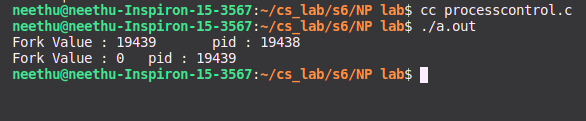
\includegraphics[scale=0.6]{img/e21.png}
        \end{figure}
\begin{verbatim}
//C program to illustrate I/O System Calls - File Manipulation

#include<stdio.h>
#include<string.h>
#include<unistd.h>
#include<fcntl.h>

int main (void){
    int fd[2];
    char buf1[12] = "hello world\n";
    char buf2[12];
    
    fd[0] = open("exp2.txt", O_RDWR);		
    fd[1] = open("exp2.txt", O_RDWR);
    
    write(fd[0], buf1, strlen(buf1));		
    write(1, buf2, read(fd[1], buf2, 12));
    
    close(fd[0]);
    close(fd[1]);
    
    return 0;
}
/*The program prints "hello world" using system call
Content of exp2.txt:
    hello world
*/
\end{verbatim}
\begin{figure}[h]
            \centering
            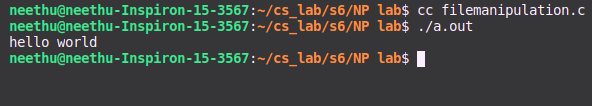
\includegraphics[scale=0.6]{img/e22.png}
        \end{figure}
\subsection{Result}
Implemented the program for system calls using C language in Ubuntu 18.04 with kernel and the above outputs were obtained.